%!TEX root = ../thesis.tex

\begin{subfigure}[b]{0.45\textwidth}
  \centering
    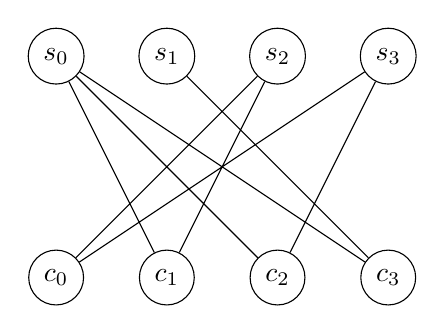
\begin{tikzpicture}
      \tikzstyle{every node}=[circle, draw]
      \foreach \i in {0, ..., 3}
      {
        \path (\i*40pt, 80pt) node (s\i) {$s_{\i}$};
      }

      \foreach \j in {0, ..., 3}
      {
        \path (\j*40pt, 0) node (c\j) {$c_{\j}$};
      }

      \draw
        (c0) -- (s2)
        (c0) -- (s3)
        (c1) -- (s0)
        (c1) -- (s2)
        (c2) -- (s0)
        (c2) -- (s3)
        (c3) -- (s0)
        (c3) -- (s1);
    \end{tikzpicture}

  \caption{\grb{}}
  \label{figure:3:a}
\end{subfigure}
\hfill
\begin{subfigure}[b]{0.45\textwidth}
  \centering
    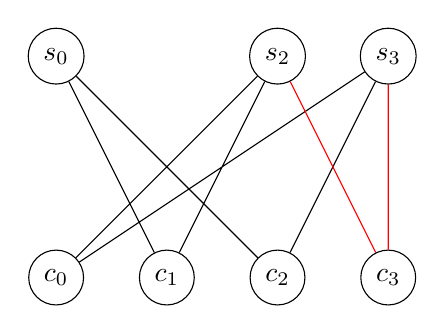
\begin{tikzpicture}
      \tikzstyle{every node}=[circle, draw]
      \foreach \i in {0, 2, 3}
      {
        \path (\i*40pt, 80pt) node (s\i) {$s_{\i}$};
      }

      \foreach \j in {0, ..., 3}
      {
        \path (\j*40pt, 0) node (c\j) {$c_{\j}$};
      }

      \draw
        (c0) -- (s2)
        (c0) -- (s3)
        (c1) -- (s0)
        (c1) -- (s2)
        (c2) -- (s0)
        (c2) -- (s3);

      \draw [red]
        (c3) -- (s2)
        (c3) -- (s3);
    \end{tikzpicture}

  \caption{\grb[0], after realizing \character[3][+]}
  \label{figure:3:b}
\end{subfigure}

\bigskip

\begin{subfigure}[b]{0.45\textwidth}
  \centering
    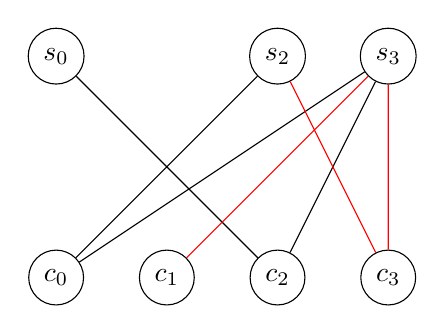
\begin{tikzpicture}
      \tikzstyle{every node}=[circle, draw]
      \foreach \i in {0, 2, 3}
      {
        \path (\i*40pt, 80pt) node (s\i) {$s_{\i}$};
      }

      \foreach \j in {0, ..., 3}
      {
        \path (\j*40pt, 0) node (c\j) {$c_{\j}$};
      }

      \draw
        (c0) -- (s2)
        (c0) -- (s3)
        (c2) -- (s0)
        (c2) -- (s3);

      \draw [red]
        (c1) -- (s3)
        (c3) -- (s2)
        (c3) -- (s3);
    \end{tikzpicture}

  \caption{\grb[1], after realizing \character[1][+]}
  \label{figure:3:c}
\end{subfigure}
\hfill
\begin{subfigure}[b]{0.45\textwidth}
  \centering
    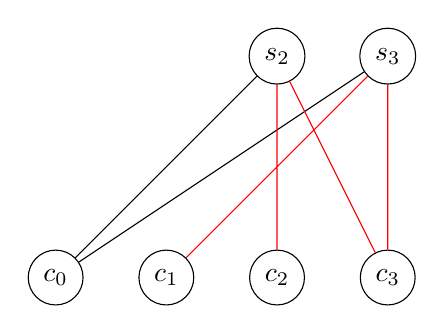
\begin{tikzpicture}
      \tikzstyle{every node}=[circle, draw]
      \foreach \i in {2, 3}
      {
        \path (\i*40pt, 80pt) node (s\i) {$s_{\i}$};
      }

      \foreach \j in {0, ..., 3}
      {
        \path (\j*40pt, 0) node (c\j) {$c_{\j}$};
      }

      \draw
        (c0) -- (s2)
        (c0) -- (s3);

      \draw [red]
        (c1) -- (s3)
        (c2) -- (s2)
        (c3) -- (s2)
        (c3) -- (s3);
    \end{tikzpicture}

  \caption{\grb[2], after realizing \character[2][+]}
  \label{figure:3:d}
\end{subfigure}

\bigskip

\begin{subfigure}[b]{0.45\textwidth}
  \centering
    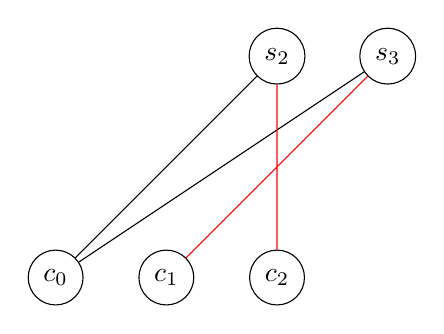
\begin{tikzpicture}
      \tikzstyle{every node}=[circle, draw]
      \foreach \i in {2, 3}
      {
        \path (\i*40pt, 80pt) node (s\i) {$s_{\i}$};
      }

      \foreach \j in {0, ..., 2}
      {
        \path (\j*40pt, 0) node (c\j) {$c_{\j}$};
      }

      \draw
        (c0) -- (s2)
        (c0) -- (s3);

      \draw [red]
        (c1) -- (s3)
        (c2) -- (s2);
    \end{tikzpicture}

  \caption{\grb[3], after realizing \character[3][-]}
  \label{figure:3:e}
\end{subfigure}
\hfill
\begin{subfigure}[b]{0.45\textwidth}
  \centering
    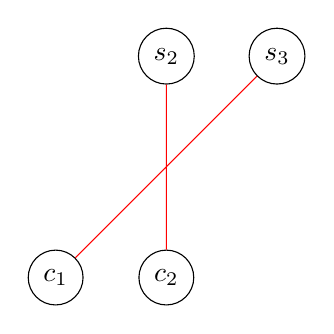
\begin{tikzpicture}
      \tikzstyle{every node}=[circle, draw]
      \foreach \i in {2, 3}
      {
        \path (\i*40pt, 80pt) node (s\i) {$s_{\i}$};
      }

      \foreach \j in {1, 2}
      {
        \path (\j*40pt, 0) node (c\j) {$c_{\j}$};
      }

      \draw [red]
        (c1) -- (s3)
        (c2) -- (s2);
    \end{tikzpicture}

  \caption{\grb[4], after realizing \character[0][+]}
  \label{figure:3:f}
\end{subfigure}

\bigskip

\begin{subfigure}[b]{0.45\textwidth}
  \centering
    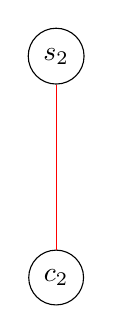
\begin{tikzpicture}
      \tikzstyle{every node}=[circle, draw]
      \foreach \i in {2}
      {
        \path (\i*40pt, 80pt) node (s\i) {$s_{\i}$};
      }

      \foreach \j in {2}
      {
        \path (\j*40pt, 0) node (c\j) {$c_{\j}$};
      }

      \draw [red]
        (c2) -- (s2);
    \end{tikzpicture}

  \caption{\grb[5], after realizing \character[1][-]}
  \label{figure:3:g}
\end{subfigure}
\hfill
\begin{subfigure}[b]{0.45\textwidth}
  \centering
    \begin{tikzpicture}
      \tikzstyle{every node}=[circle, draw]
      \foreach \i in {}
      {
        \path (\i*40pt, 80pt) node (s\i) {$s_{\i}$};
      }

      \foreach \j in {}
      {
        \path (\j*40pt, 0) node (c\j) {$c_{\j}$};
      }
    \end{tikzpicture}

  \caption{\grb[6], after realizing \character[2][-]}
  \label{figure:3:h}
\end{subfigure}
